\documentclass[10pt,a4paper]{book}
\usepackage[utf8]{inputenc}
\usepackage{amsmath}
\usepackage{amsfonts}
\usepackage{amssymb}
\usepackage{wasysym}
\usepackage{multicol}
\usepackage{hyperref}
\usepackage{tabularx}
\usepackage{subfig}
\usepackage{tikz}
\usepackage[ruled, lined, longend]{algorithm2e}
\usepackage[shortlabels]{enumitem}
\usepackage{textcomp}
\usepackage{chemfig}

\setlength{\parindent}{20pt}
\hypersetup{
    colorlinks,
    citecolor=black,
    filecolor=black,
    linkcolor=black,
    urlcolor=darkgray
}

\newcommand{\R}{\mathbb{R}}
\newcommand{\N}{\mathbb{N}}
\newcommand{\Z}{\mathbb{Z}}
\newcommand{\ind}{\hspace*{\parindent}}

\title{Chimie générale \vspace{0.2cm} - Notes and Summary}
\author{Mahel Coquaz}
\date{Spring Semester 2025}

\begin{document}
\maketitle
\tableofcontents
\newpage
%\part*{Atomistique}
\chapter{Atomistique}
\section{L'atome}
\paragraph{Le modèle de l'atome}
Les molécules sont constituées d'atomes qui se partagent des électrons, ces liaisons chimiques dépendent des électrons externes et donc de la configuration électronique des atomes.
Le modèle de l'atome:
\begin{enumerate}
\item Modèle Rutherford
\begin{itemize}
\item L'électron tourne autour du noyau de manière aléatoire.
\item Rendu obsolète.
\end{itemize}
\item Modèle Schrödinger
\begin{itemize}
\item On ne sait pas précisément où est l’électron, c'est un modèle mathématique.
\item Modèle actuel, quantique.
\end{itemize}
\item Modèle Bohr
\begin{itemize}
\item L'électron tourne autour du noyau selon des orbites précises correspondant à des niveaux énergétiques.
\item Physiquement faux mais toujours utilisé pour décrire certaines propriétés atomiques.
\end{itemize}
\item Modèle Thomson
\begin{itemize}
\item Charge positive distribuée uniformément sur une sphère. Les électrons sont distribués de manière à contrebalancer cette charge.
\item Obsolète.
\end{itemize}
\end{enumerate}
\newpage
\paragraph{L'atome et ses constituants} L'atome est constitué de:
\begin{itemize}
\item Le noyau de diamètre \textasciitilde 1 femtomètre (10$^{-15}$m)
\begin{itemize}
\item Protons
\begin{itemize}
	\item Masse: 1.0073 uma\footnote{1 uma = 1.66054 $\times$ 10$^{-24}$ g}
	\item Charge: Positive (+1) 
\end{itemize}
\item Neutrons
\begin{itemize}
	\item Masse: 1.0087 uma
	\item Charge: Neutre (+0) 
\end{itemize}
\end{itemize}
\item Le nuage électronique de diamètre 1 {\AA}ngstrom (1 {\AA} = 10$^{-10}$m)
\begin{itemize}
\item Électrons
\begin{itemize}
	\item Masse: 5.486 $\times$ 10$^{-4}$ uma
	\item Charge: Négative (-1) 
\end{itemize}
\end{itemize}
\end{itemize}
\paragraph{Les atomes d'un élément} Les protons, neutrons, électrons sont les mêmes pour chaque élément. \\ 
Un élément est caractérisé par son nombre de protons (numéro
atomique) \\
Un atome électriquement neutre comporte le même nombre d’électrons
que de protons.\\
Un atome contenant un nombre différent d’électrons et
de protons est appelé ion (monoatomique). On distingue les cations (chargés positivement) des anions (chargés négativement). \\ 
Les isotopes d’un même élément diffèrent par leur nombre de
neutrons. Les isotopes d’un élément ont la même réactivité chimique.\\
La notation d'un atome est la suivante: \\
\textbf{\[{X_A^Z} \hspace{1cm} { }_{Z numero atomique}^{A nombre de masse}\]} %need to fix later
\section{Structure de l'atome}
\subsection{La conception (semi)quantique}
\paragraph{Les travaux de Niels Bohr} Chez Bohr l'énergie d'un électron est quantifiée: ce sont les niveaux d'énergie. \\
Les valeurs permises des niveaux d'énergie sont définies par:
\begin{displaymath}
E_n = - \frac{R_h}{n^2}
\end{displaymath}
$R_h$ = 2.179$\times$10$^{-18}$ J = 13.6eV\footnote{1eV = 1.602$\times$10$^{-19}$C $\times$ 1V}\\
n $\in$ $\mathbb{N}$ \par
Chaque valeur possible pour l'énergie correspond à une trajectoire et une distance noyau-électron. Le niveau n = 1 correspond au niveau d'énergie le plus bas et à l'orbite la plus proche du noyau, c'est \textbf{l'état fondamental}.\par
Les changements d'énergie de l'électron s'opèrent par sauts discontinus et le passe dans un \textbf{état excité}. Tant qu’un électron demeure à un niveau d’énergie donné, il ne peut pas émettre d’énergie sous forme de rayonnement électromagnétique. \par
Lorsque $lim_{n \rightarrow \infty}$ $E_n$ = 0, c'est \textbf{l'ionisation}. \par
\begin{displaymath}
{\Delta}E_n = E_{n_{arriv\acute{e}}} - E_{n_{d\acute{e}part}}
\end{displaymath}
\subsubsection{Résumé du modèle de Bohr}
\begin{enumerate}
\item On a un atome stable.
\item L'énergie d'un électron est quantifié (et quantifiable).
\item Bonne (mais imparfaite) explication du spectre de l’atome d’hydrogène et des atomes avec un seul électron.
\begin{displaymath}
E_n = -\frac{{Z^2}{R_h}}{n^2}
\end{displaymath}
\end{enumerate}
Limitations:
\begin{enumerate}
\item N'explique pas la structure fine des spectres d'hydrogène (manque une information supplémentaire: le spin)
\item Ne s'applique pas aux atomes avec plusieurs électrons (car les intéractions entre électrons sont décrites par la valeur efficace de Z)
\end{enumerate}
\begin{displaymath}
E_n = -\frac{{Z_{eff}^2}{R_h}}{n^2}
\end{displaymath}
\begin{center}
\begin{tabular}{ | m{5cm} | m{5cm}| m{5cm} | } 
  \hline
  Bohr & Schrödinger \\ 
  \hline
  L’électron est décrit comme une particule avec une trajectoire précise. & L'électron est décrit par une fonction d’onde $\psi$ liée à la probabilité de présence. \\ 
  \hline
  Lois de la mécanique classique selon Newton. & Lois de la mécanique quantique selon Schrödinger. \\ 
  \hline
  Case quantique: définit seulement le niveau d’énergie de l’électron (orbite) & Orbitale: définit à la fois le niveau d’énergie et la probabilité de présence de l'électron. \\
  \hline
\end{tabular}
\end{center}
\subsection{Le modèle de Schrödinger}
\paragraph{Les solutions de l'équation de Schrödinger}
\begin{enumerate}
\item La résolution analytique de l’équation de Schrödinger pour l’atome d’hydrogène ou numérique pour les atomes à plusieurs électrons n’est pas au programme de ce cours.
\item Les diverses solutions de l’équation de Schrödinger sont des orbitales $\Psi_n$, l, $m_l$ définies par 3 nombres entiers (appelés nombres quantiques): n, l, $m_l$ .
\item Une orbitale est une expression mathématique. La représentation géométrique des orbitales n’est possible que pour un pourcentage défini de probabilité de présence d’un lectron (par exemple 90\%) car l’expression mathématique de l’orbitale n’est pas finie.
\item  Pour définir un électron dans une orbitale, nous avons besoin d’un $4^{\grave{e}me}$ nombre quantique: le spin $m_s$. \label{spin}
\item  La configuration électronique nous permet de déterminer le nombre l'électrons de valence ( les électrons de la couche externe avec le nombre quantique n le plus grand).
\end{enumerate}
\subsubsection{Les nombres quantiques}
\paragraph{Les quatres nombres quantiques} décrivent l'état d'un électron (énergie, région d'espace:
\begin{enumerate}
\item \textbf{n} : principal (n $\geq$ 1)
\item \textbf{l} : secondaire (0 $\leq$ l $\leq$ n - 1) 
\item \textbf{$m_l$} : magnétique (-l $\leq$ $m_l$ $\leq$ l)
\item \textbf{$m_s$} : spin ($\pm \frac{1}{2}$)
\end{enumerate}
\paragraph{Principe d'exclusion de Pauli} Il ne peut exister que deux atomes définis par le même groupe de quatre nombres quantiques. Une orbitale comprenant au maximum deux électrons \textbf{de spins \textit{opposés}} \label{eq:1}
% slide 20 add 2n^2 (nombre total d'électrons si n est plein ou...? + schema maybe
\subsubsection{Configuration électronique des atomes}
La configuration électronique d'une atome décrit la distribution des électrons dans ces diverses orbitales.
\paragraph{Notation spdf}
\begin{itemize}
\item Niveau d'énergie \textit{n} $\rightarrow$ désigné par un nombre
\item Type d'orbitale \textit{l} $\rightarrow$ désigné par une lettre (s, p, d, f)
\item Nombre d'électrons dans l'orbitale $\rightarrow$ désigné par un exposant
\end{itemize}
\begin{displaymath}
1s^22s^22p^3
\end{displaymath}
$_\nearrow$ 2 électrons dans l'orbitale 1s \\
$\rightarrow$ 2 électrons dans l'orbitale 2s \\
$^\searrow$ 3 électrons dans l'orbitale 2p 
\paragraph{Notation spdf étendue} on peut distribuer des électrons dans les orbitales, on les représente dans des $\ll$\textbf{cases quantiques}$\gg$.
\begin{displaymath}
1s^22s^22p_x^12p_y^12p_z^1
\end{displaymath}
Se traduit par :
\begin{center}
\begin{tabular}{| c | c | c | c | c |}
\hline
$\uparrow\downarrow$ & $\uparrow\downarrow$ & $\uparrow$ & $\uparrow$  & $\uparrow$ \\
\hline
\end{tabular} \\
\begin{tabular}{| c | c | m{1.5cm}|}
\hline
1s & 2s & 2p \\
\hline
\end{tabular}
\end{center}
\subsubsection{Répartition des électrons autour du noyau}
\begin{itemize}
\item Répartition en couches (n = 1, 2, 3...) et sous couches (s, p, d...)
\item Le remplissage des couches et sous couches se fait selon la séquence d'énergie croissante (princide de construction d'Aufbau)
\item L'état fondamental se construit à partir de:
\begin{itemize}
	\item La règle d'exclusion de Pauli \ref{eq:1}
	\item La règle de Hund : L'arrangement le plus stable est celui contenant le plus de spin parallèles.
\end{itemize}
\end{itemize}
\par À l'état fondamental, les électrons occupent les orbitales correspondant aux \textbf{plus bas niveaux d'énergie possible}.
\subsubsection{La règle de Klechkowski/l'Aufbau}
\begin{figure}[h!]
\begin{center}
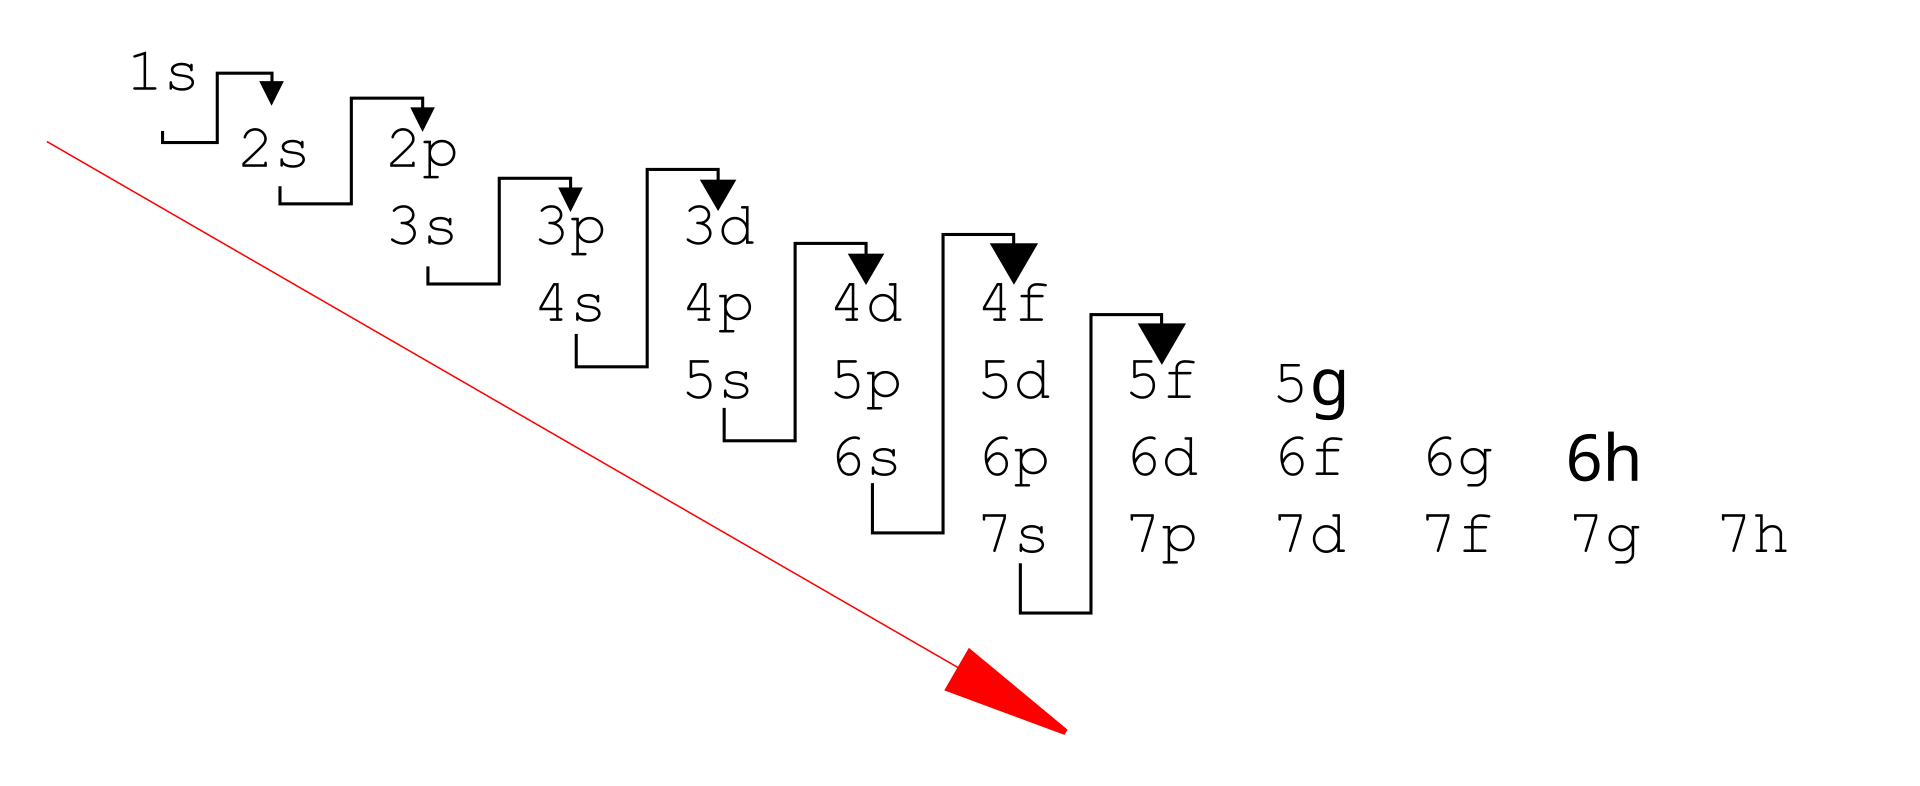
\includegraphics[scale=0.15]{./assets/klechkowski_rule.png}
\caption{Règle de Klechkowski}
\label{fig:klechkowski}
\end{center}
\end{figure}
\paragraph{Exceptions à la règle de l'Aufbau} Il existe certaines exceptions à ces règles \textbf{ELLES NE SONT PAS AU PROGRAMME}, mais il faut être au courant de leur existence.
\begin{figure}[h!]
\begin{center}
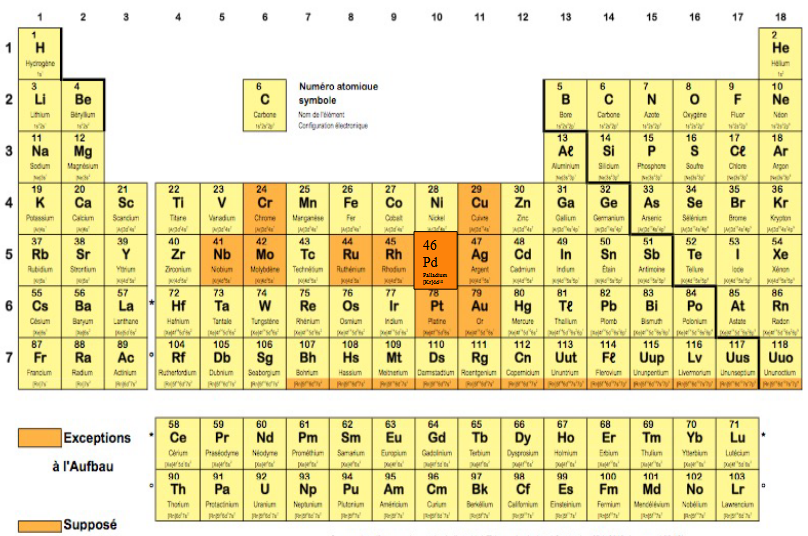
\includegraphics[scale=0.45]{./assets/aufbau_exceptions.png}
\end{center}
\caption{Exceptions à l'Aufbau}
\label{fig:exceptions}
\end{figure}
\newpage
\subsection{Classification périodique des éléments}
\paragraph{Classification selon Z} La classification des éléments se fait selon l'ordre croissant du numéro atomique \textbf{Z}. Les 92 premiers éléments sont dits "naturels" tandis que les éléments de 93 à 118 ont été préparés artificiellement. \par
Les colonnes sont désignées par un numéro de 1 à 18 ou par des symboles (IA, IIA, IIB...). Les éléments d'une même colonne constituent un groupe et portent un nom particuliers (i.e. métaux alcalins, gaz rares, halogènes, alcalino-terreux...). Ils ont également le \textbf{même nombre d'électrons de valence\footnote{électrons sur la dernière couche électronique de l'atome}}. \par 
Les lignes sont appelées \textbf{périodes}, elles sont numérotées de 1 à 7.
\paragraph{Le rayon atomique} Il existe plusieurs définitions du rayon atomique: par le calcul et la demi-distance entre centres d'atomes voisins (données expérimentales). \par
Le rayon atomique augmente en bas le long d'un groupe et diminue de gauche à droite le long d'une période ($Z_{eff}$\footnote{Zeff est la charge effective ressentie par l’électron le plus éloigné du noyau. Elle dépend de la charge du noyau et des autres électrons de l’atome.} $\nearrow$):
\begin{displaymath}
r \propto \frac{n^2}{Z_{eff}}
\end{displaymath}
\subsubsection{Charge nucléaire effective $Z_{eff}$}
\begin{displaymath}
Z_{eff} = Z - \delta
\end{displaymath}
avec $Z_{eff}$ la charge nucléaire effective, Z la charge nucléaire réelle et $\delta$ l'effet d'écran des électrons.
\begin{figure}[h!]
\begin{center}
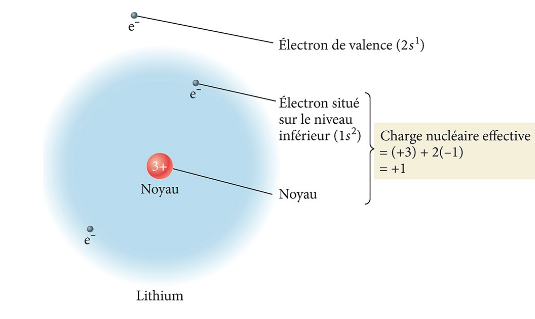
\includegraphics[scale=0.75]{./assets/zeff_example.png}
\end{center}
\caption{Exemple de $Z_{eff}$}
\label{fig:Zeff}
\end{figure}
\paragraph{L'énergie d'ionisation} Elle diminue de haut en bas d’un groupe et augmente le long d’une période.
\begin{displaymath}
IE = -E_n = \frac{Z_{eff}^2R_h}{n^2}
\end{displaymath}
\section{L'électronégativité}
\paragraph{Prédiction des propriétés des éléments} \hypertarget{electronegativity}{L'éléctronégativité} traduit le pouvoir \textbf{electro-attracteur} d'un atome lorsqu'il est engagé dans une liaison. \par 
Cette échelle arbitraire allant de 0 à 4 est sans unité. \\
L'électronégativité détermine le partage des électrons dans une liaison: les électrons vont se diriger vers l'atome le plus électronégatif.
\subsection{Récapitulatif des tendances périodiques}
\begin{figure}[h!]
\begin{center}
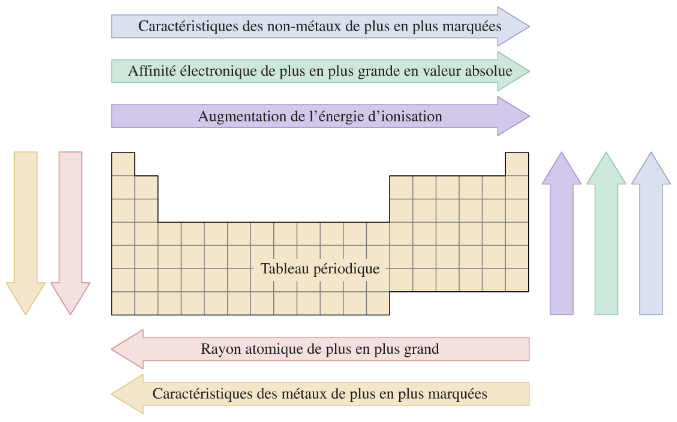
\includegraphics[scale=0.75]{./assets/recap_tendencies.png}
\end{center}
\caption{Récapitulatif des tendances périodiques}
\label{fig:recap}
\end{figure}
\chapter{Liaisons chimiques}
\section{Introduction}
\paragraph{Qu'est-ce qu'une liaison chimique ?} Une liaison chimique est un ensemble de forces électriques assurant la cohésion des molécules, elles résultent du partage du \textbf{partage d'électrons entre les atomes}. \par
Une liaison chimique correspond toujours à un \textbf{minimum énergétique}, elle se forme si l'arrangement des atomes final à une énergie \textit{plus faible} que la des énergies des atomes séparés. Par conséquent la formation de liaisons à pour conséquence \textbf{un dégagment d'énergie}.
\subsection{Les types de liaisons}
\paragraph{Liaison ionique} Une liaison entre \textbf{deux ions de signes \textit{opposés}} avec un passage d'électrons d'un atome à l'autre.\\ %need precisions 
\textbf{Cette liaison requiert une grande différence d'électronégativité !} ($\Delta$EN $>$ 1.7)
\paragraph{Liaison covalente} Cette liaison résulte d'un partage d'électron(s) entre deux atomes d'électronégativité semblable. Elles se distinguent entre les liaisons covalentes \textit{polaires} et \textit{apolaires}. \par
La force électroattractrice d'un atome est quantifié par son \hyperlink{electronegativity}{électronégativité}. Tant que $\Delta$EN $<$ 0.4 on parle de \textbf{liaison covalente non polaire} (ou covalente pure si $\Delta$EN = 0 comme pour $H_2$) , ensuite  entre 0.4 $<$ $\Delta$EN $<$ 1.7 on parle de \textbf{liaison covalente polaire} 
\paragraph{Liaison métallique} Il s'agit du partage des électrons de valence entre tous les atomes d'un métal (électronégativité faible), les électrons ainsi libres permettent la conductivité électrique !
\newpage
\section{Théorie de Lewis}
\paragraph{Les fondements de la théorie de Lewis} Selon Lewis les \textbf{électrons de valence} (électrons avec la valeur \textit{n} la plus grande) jouent un rôle fondamental dans les liaisons chimiques. \par
Lorsque les atomes perdent, recoivent ou partagent des électrons au cours de liaisons ils vont \textit{en général} acquérir la configuration électronique d'un \textbf{gaz noble}: ce sont les règles du \textbf{duet et de l'octet}\footnote{Seuls l'hydrogène (H), le lithium (Li) et le béryllium (Be) observent la règle du duet et prennent la forme de l'hélium (He)}.

\subsection{La représentation de Lewis}
La représentation de Lewis se concentre sur la couche externe que l'on représente simplifiée à l'aide de points symbolisant les \textbf{électrons de valence}. Les quatres premiers électrons sont représentés isolés, puis on groupe les électrons additionnels sous la forme de \textbf{doublets}.
% ajouter la partie sur les liaisons ioniques
\subsubsection{Méthodologie de Lewis (liaisons covalentes)}
\begin{enumerate}
\item Dénombrer les électrons de valence des tous les atomes de la molécule
\item Dessiner le \textbf{squelette} de la molécule en reliant les atomes les uns aux autres par une paire d'électrons. L'atome le \textbf{moins électronégatif} occupe la place \textbf{centrale}.
\item Placer les électrons restants sur l'atome central.
\item Si le nombre d'électrons disponibles est insuffisant il faut introduire des \textbf{liaisons multiples} et attribuer les charges de l'ion
\end{enumerate}
\textbf{Exemple: NH$_3$}
\begin{center}
\begin{enumerate}
\item \charge{0=\.,90=\:,180=\.,270=\.}{N}
\item \chemfig{\charge{90=\:}{N}(-[:0]H)(-[:180]H)(-[:270]H)}
\item Pas nécessaire ici.
\item Pas nécessaire ici.
\end{enumerate}
\end{center}
\textbf{Exemple: AsCl$_3$}
\begin{enumerate}
\item On dénombre le nombre d'électrons de valence:
\begin{itemize}
	\item 5 pour l'As
	\item 3$\times$7 pour Cl$_3$
\end{itemize}
\item On dessine le squelette et on relie: \chemfig{As(-[:45]Cl)(-[:135]Cl)(-[:270]Cl)}
\item On complète les octets (24 électrons utilisés) : \chemfig{As(-[:45]\charge{315=\|,45=\|,135=\|}{Cl})(-[:135]\charge{225=\|,45=\|,135=\|}{Cl})(-[:270]\charge{0=\|,180=\|,270=\|}{Cl})}
\item Placer les électrons restants sur l’atome central: \chemfig{\charge{90=\|}{As}(-[:0]\charge{0=\|,90=\|,270=\|}{Cl})(-[:180]\charge{90=\|,180=\|,270=\|}{Cl})(-[:270]\charge{0=\|,180=\|,270=\|}{Cl})}
\item %TODO add note
\end{enumerate}
\paragraph{Limites de la représentation de Lewis} Il s'agit d'une représentation empirique, cependant couplée à la représentation VSPR (voir \ref{VSPR}) elle permet une représentation géométrique de la forme de la molécule une estimation de sa polarité et de sa réactivité chimique. \\
Par exemple la règle de l’octet (ou doublet (H, He, Li, Be)) ne s’applique pas à tous les éléments/molécules !
\begin{itemize}
\item Hypovalence
\item Hypervalence
\item Les molécules à nombre impair d'électrons de valence (i.e. NO qui possède 11 électrons de valence)
\end{itemize}
De plus certaines propriétés comme le \textbf{paramagnétisme} doivent être décrites avec une représentation plus précise des électrons (la notion du spin voir \ref{spin}).

\section{Représentation VSEPR} \label{VSPR}
\subsection{Le modèle RPEV ou VSPER} Le modèle de la Répulsion des Paires d’Electrons de Valence (RPEV) ou le Valence-Shell Electron-Pair Repulsion (VSEPR). \\
Lorsque l'on considère un atome, les paires d’électrons liantes et non liantes se placent de telle sorte à \textbf{minimiser} leur énergie de répulsion, la forme de la molécule dépend donc des atomes liés à \textbf{l'atome central}.
\begin{displaymath}
AX_nE_m
\end{displaymath}
A: atome central \\
n: nombre d’atomes liés à l’atome central \\
m : nombre de doublets libres de l’atome central \par
Les molécules de types AX$_n$E$_m$ ont une description \textbf{électronique} dépend des \textbf{atomes liés} et des \textbf{doublets non liants}. Cependant la \textbf{géométrie moléculaire} \textit{ignore} ces derniers.
\paragraph{Géométrie des molécules} On définit $\alpha_1$ et $\alpha_2$ les angles axiaux et équatoriaux des molécules\footnote{Pour des raisons de concision on se contentera ici de tableaux récapitulants les structures ;)}.
\begin{figure}[h!]
\begin{center}
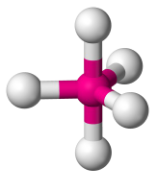
\includegraphics[scale=0.75]{./assets/geometry_example.png}
\caption{Example de géometrie avec $\alpha_1$ = 120° et $\alpha_2$ = 90°}
\label{fig:geometry_ex}
\end{center}
\end{figure}
\begin{figure}[h!]
\begin{center}
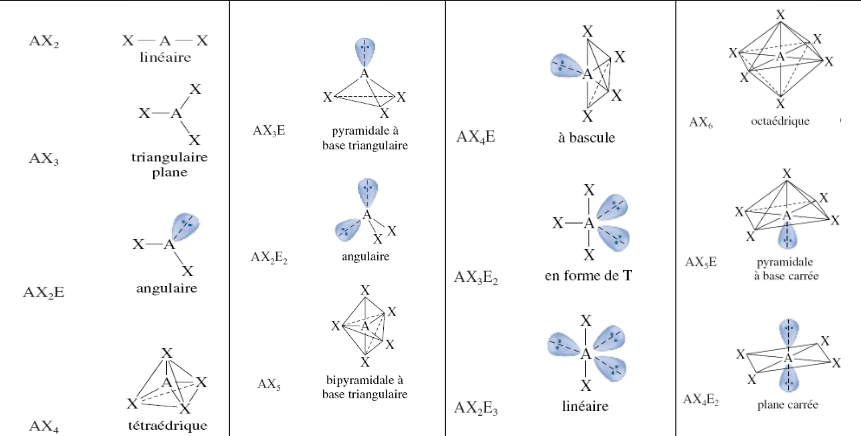
\includegraphics[scale=0.65]{./assets/geometry_table.png}
\caption{Tableau des géométries}
\label{fig:geometry_table}
\end{center}
\end{figure}
%TODO add the two other tables in a nicer way
\subsection{Polarité des molécules}
\title{Le moment dipolaire:}
\begin{displaymath}
\mu = \delta \times l
\end{displaymath}
$\delta$: charge électrique partielle résultant de la polarisation \\
$l$: longueur de la liaison\\
Par exemple pour HCl:\\
\begin{center}
$\delta+$ \; \; $\delta-$ \\
\chemfig{H(-[:0]Cl)}
\end{center}
Avec $\mu$ = 1,02D\footnote{1 D (Debye) = 3,36 x 10$^{-30}$ C$\cdot$m}
\paragraph{Géométrie et polarité} Les molécules dites \textbf{symétriques} son \textbf{apolaires} (la somme vectorielle des moments dipolaires est nulle) même si les liaisons individuelles sont polaires \\
À l'inverse les molécules dites \textbf{asymétriques} conduit (en cas de présence de liaisons individuelles polaires) à une molécule \textbf{polaire}.

\section{Approche quantique}
\subsection{Recouvrement des orbitales}
\paragraph{Théorie de la liaison de valence} Une liaison covalente résulte de la formation d’un doublet d’électrons de spins opposés dans la région du recouvrement de deux orbitales atomiques. \\
Exemple, formation d'H$_2$:
\begin{enumerate}
\item Deux atomes d’hydrogène se rapprochent l’un de l’autre. Ils renferment chacun un électron dans l’orbitale 1s de spin opposés.
\item A une certaine distance, les orbitales commencent à se chevaucher : recouvrement des orbitales 1s. \\
La région du recouvrement contient alors 2 électrons de spins opposés.
\item Augmentation de la densité électronique dans la région située entre les 2 noyaux : maintient ensemble les 2 noyaux.
\end{enumerate}
\subsection{Hydration}
Exemple, le méthane CH$_4$:
\begin{center}
La configuration de C à l'état fondamental: \\ \vspace{0.5cm}
\begin{tabular}{| c | c | c | c | c |}
\hline
$\uparrow\downarrow$ & $\uparrow\downarrow$ & $\uparrow$ & $\uparrow$  & \: \\
\hline
\end{tabular}\\
1s \quad 2s \quad \qquad 2p
\end{center}
\par On constate que l'orbitale 2p contient deux électrons non appariés $\rightarrow$ on prédit alors que la molécule la plus simple est CH$_2$. Cependant CH$_2$ n'est pas stable, l'hydrocarbure stable le plus simple est CH$_4$. \par
Cependant pour construire CH$_4$ on a besoin de 4 électrons non appariés. Il faut donc:
\begin{enumerate}
\item Promouvoir des électrons dans les orbitales d'énergie supérieure.
\item Il faut que les quatre orbitales de l’atome de C qui vont se recouvrir avec l’orbitale 1s des atomes d’hydrogène soient identiques.
\end{enumerate}
C'est \textbf{l'hybridation} des orbitales \textbf{2s} et \textbf{2p} 
\end{document}
